% コンパイル方法: lualatex filename.tex
\RequirePackage{plautopatch}

\documentclass[a4paper, 10pt]{ltjsarticle}


% マージン設定
\usepackage[top=20mm, bottom=20mm, left=20mm, right=20mm]{geometry}

% LuaLaTeX用日本語対応パッケージ
\usepackage{luatexja}
\usepackage{luatexja-fontspec}

% 必要なパッケージ
\usepackage{fontspec}
\usepackage{titlesec}
\usepackage{graphicx}
\usepackage{amsmath}
\usepackage{amssymb}
\usepackage{hyperref}
\usepackage[english, japanese]{babel}
\usepackage{multicol} % 二段組用パッケージ
\usepackage{indentfirst}
\usepackage{tikz} % カスタム点線用
\usepackage{authblk} % 著者・所属パッケージ
\usepackage{here}
\usepackage{caption}

% \setmainfont[Ligatures=TeX]{Times New Roman}
% \setmainjfont[BoldFont=MS Gothic]{MS Mincho}

\renewcommand{\baselinestretch}{0.95}

% セクション見出しのカスタマイズ
\titleformat{\section}
  {\fontsize{10pt}{10pt}}
  {\thesection.}
  {1em}{}

\titleformat{\subsection}
  {\fontsize{10pt}{10pt}}
  {\thesubsection}
  {1em}{}

\titleformat{\subsubsection}
  {\fontsize{10pt}{10pt}}
  {\thesubsubsection}
  {1em}{}

  \setlength{\parindent}{1em}
% \setlength{\belowcaptionskip}{1em} % キャプション下の余白を -10pt に設定



\titlespacing*{\section}{0em}{1em}{0em}
\titlespacing*{\subsection}{0em}{1em}{0em}

\pagestyle{empty}


\begin{document}

% \setlength{\abovedisplayskip}{1em}
% \setlength{\belowdisplayskip}{1em}
\setlength{\columnsep}{7.5mm}

\twocolumn[
    \begin{center}
        {\vspace{-1em}}

        {\fontsize{15pt}{15pt}\selectfont{クロスレイヤシミュレータ開発における無線LANシミュレータの開発}}

        {\vspace{1.3em}}

        {\fontsize{13pt}{13pt}\selectfont{Development of a Wireless LAN Simulator for Cross-Layer Simulator Development }}
    \end{center}

    \vspace{0.1em}

    \begin{flushright}
      {\fontsize{11pt}{11pt}\selectfont{T5-16 \; 下沢亮太郎\\}}
      {\fontsize{11pt}{11pt}\selectfont{指導教員 \; 設樂勇}}
    \end{flushright}

    \vspace{1em}

    \thispagestyle{empty}
]

\section{緒言}
近年,無線通信端末利用者の急増に伴い様々な場所で無線通信システムが利用されており,今後も利用の増加と発展が見込まれている.近年の無線通信技術の進歩に伴い,システムが高機能化・複雑化しており,従来のようにレイヤごとに独立した性能評価を行う手法では通信全体の実用的な評価を十分に行うことが困難になりつつある.

そのため,通信全体をクロスレイヤで評価できる計算機シミュレータの開発が求められている.本研究ではクロスレイヤシミュレータにおけるMACレイヤの挙動をシミュレートする機能を開発を行い,その有効性を評価した.


\section{提案手法}

\subsection{CSMA/CA}

\begin{figure}[H]
  \centering
  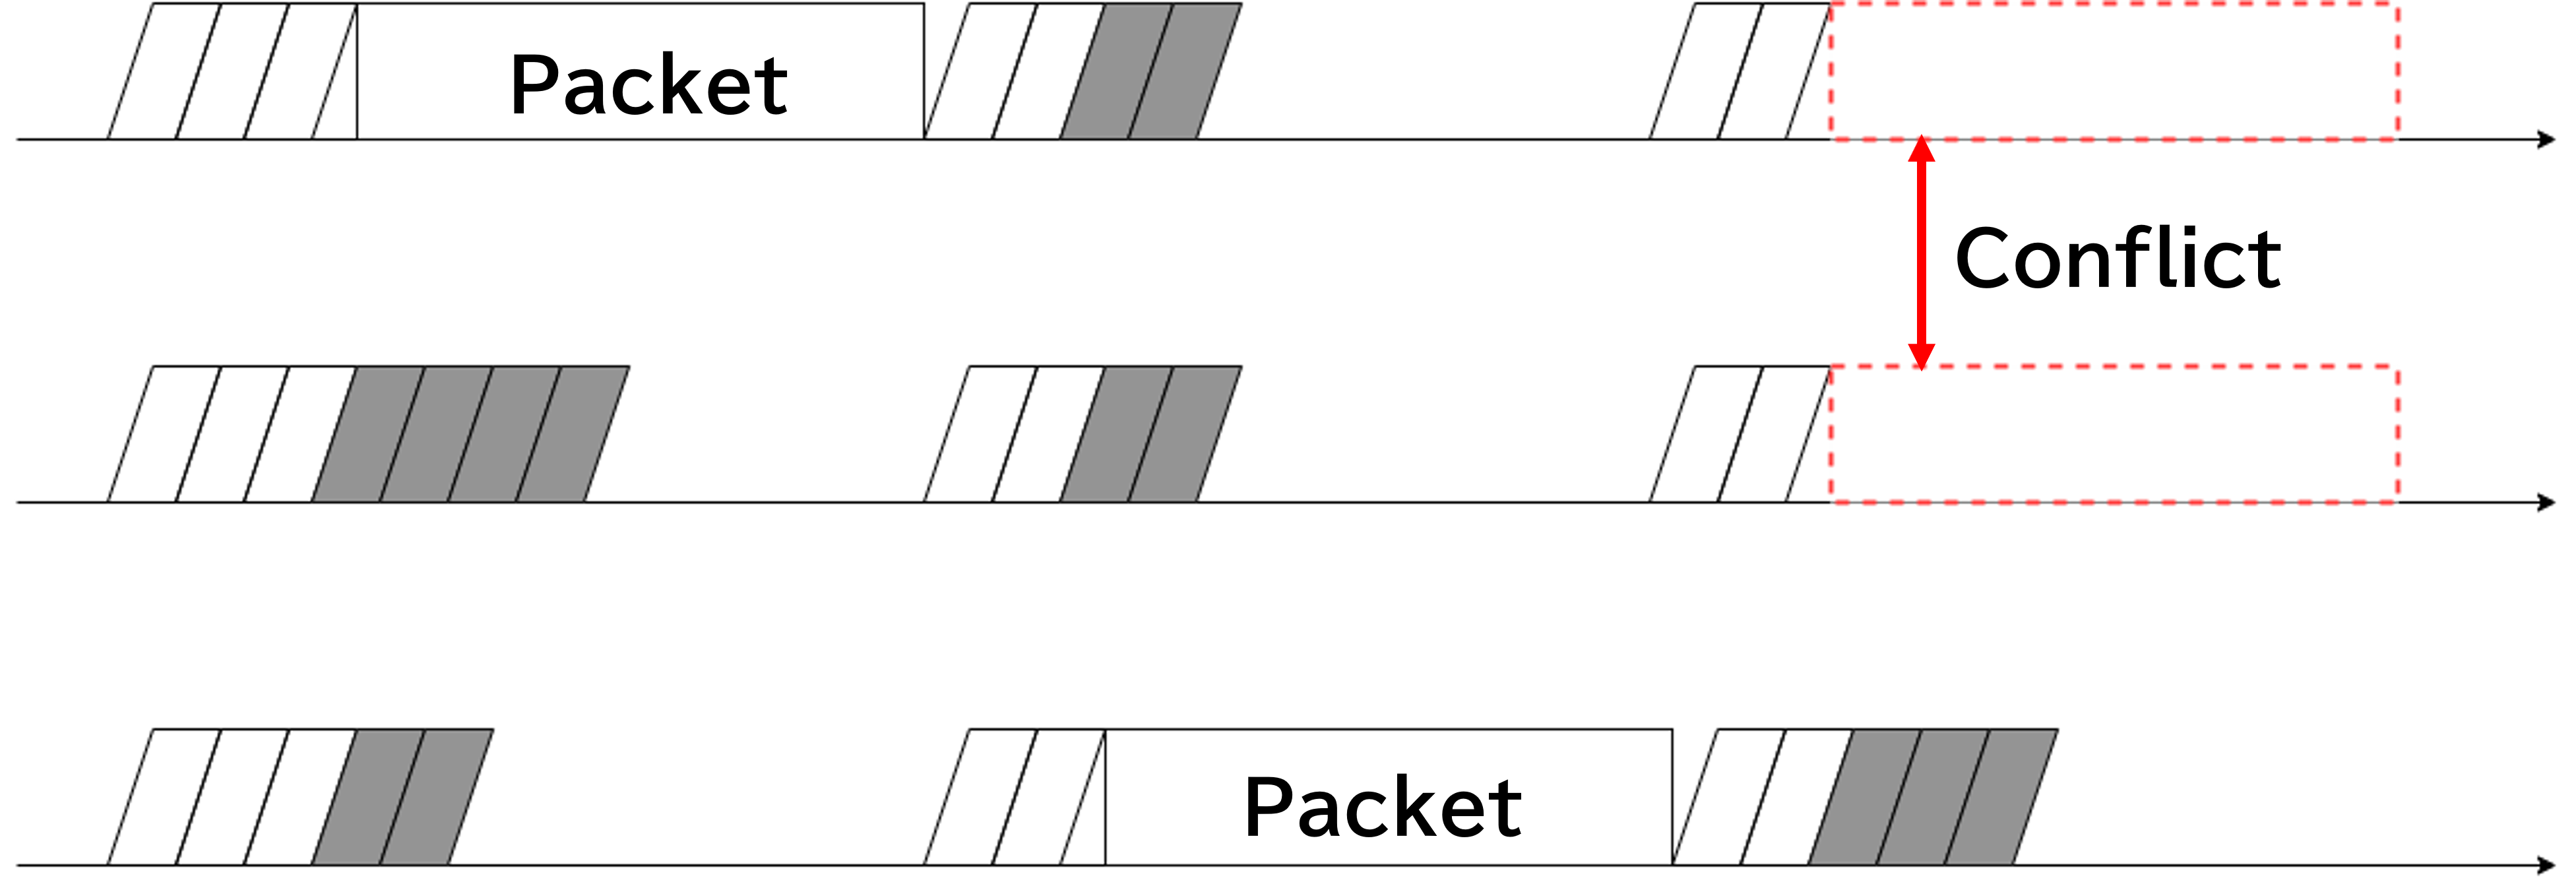
\includegraphics[width=1\columnwidth]{./assets/csmaca-1.png}
  \caption{CSMA/CA概要}
\end{figure}

\subsubsection{CW(Contention Window)}

再送回数を$n$とするとCWの最大値は

\begin{align}
  \text{cw\_max} &= 2^{4 + n} - 1
\end{align}

となり,スロット数は

\begin{align}
  \text{slots} &= \mathrm{randint}(1, \; \min(\text{cw\_max}, \; 1023))
\end{align}

で定義される.


\subsection{パケット構成モデル化}
\begin{figure}[H]
  \centering
  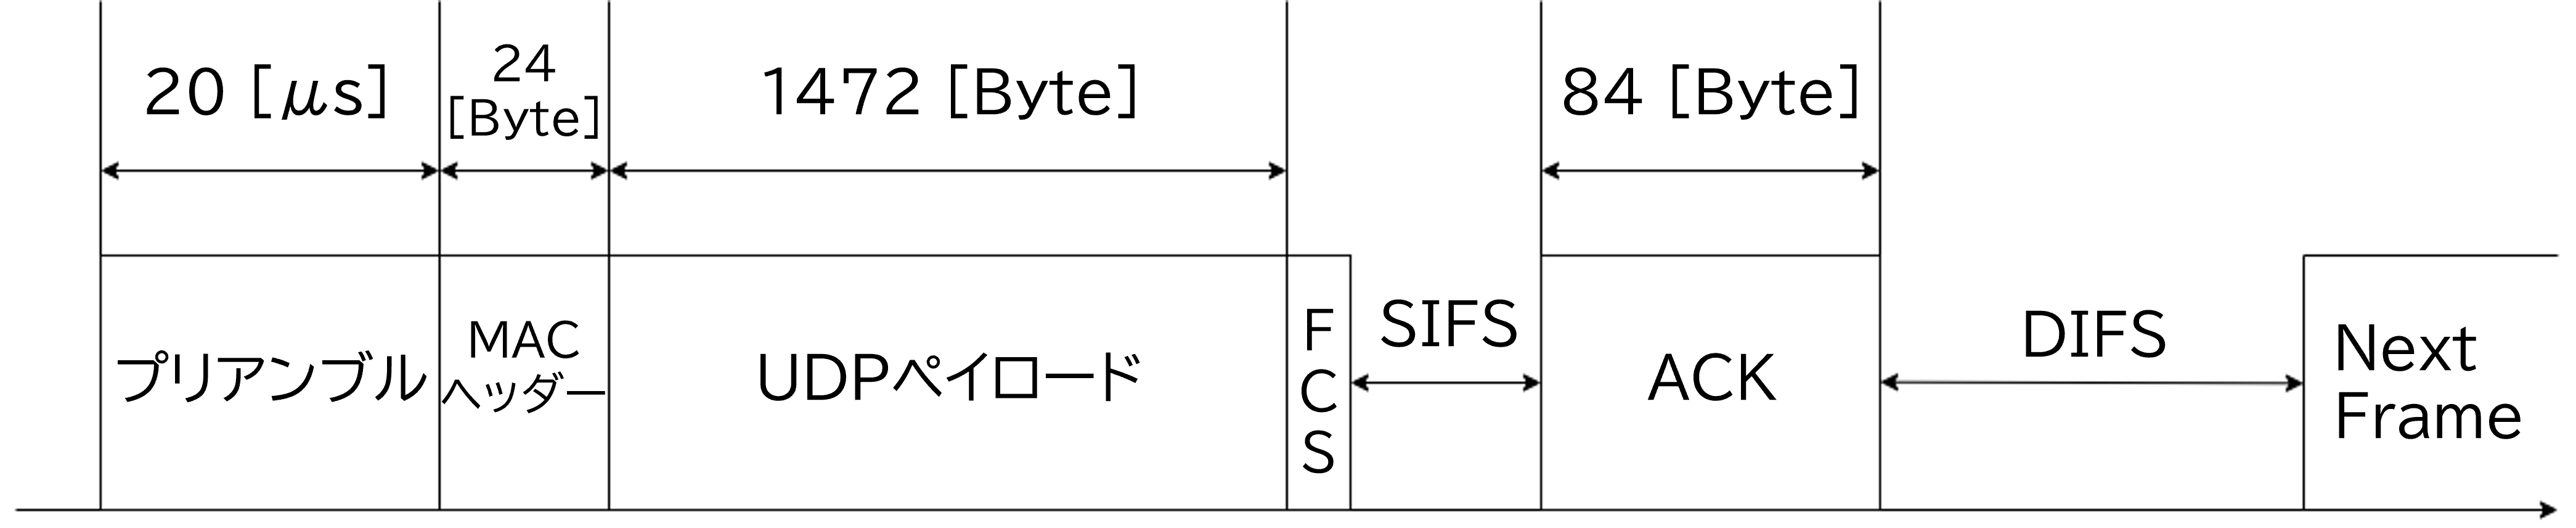
\includegraphics[width=1\columnwidth]{./assets/packet.png}
  \caption{モデル化されたパケット構成図}
\end{figure}


\subsection{User class(必要だったら)}


\section{結果}
図\ref{fig:simulation-result}に,横軸を端末数,縦軸をスループットとし,シミュレーション結果と理論値を併せてプロットしたグラフを示す.
% 横軸に端末数,縦軸にスループットを取ったグラフを図\ref{fig:simulation-result}に示す.


\begin{figure}[H]
  \centering
  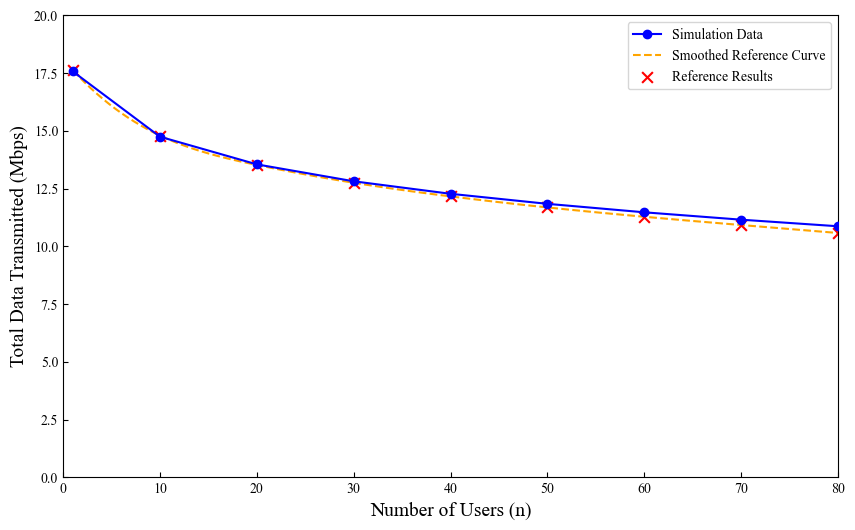
\includegraphics[width=1\columnwidth]{./assets/g3.png}
  \caption{シミュレーション結果}
  \label{fig:simulation-result}
\end{figure}

\section{結言}
本研究では,クロスレイヤシミュレータの一部である無線LANシミュレータを開発し,CSMA/CAを中心とした動作のモデル化と検証を行った.

現在の方法では通信が連続して行われているが,ポアソン分布に従った時間だけ離すことで実際の通信頻度に近い状況を再現することや,各ステーションに距離の概念を持たせて自由空間伝搬による減衰を考慮することが今後の課題である.

\begin{thebibliography}{9}
  \bibitem{midori}守倉正博, 久保田周治, 『インプレス標準教科書シリーズ 改訂三版802.11 高速無線LAN教科書』, 株式会社インプレスコミュニケーションズ, 2016年
  \bibitem{paper}Y. Morino, T. Hiraguri, H. Yoshino, K. Nishimori, T. Matsuda, ``A Novel Collision Avoidance Scheme Using Optimized Contention Window in Dense Wireless LAN Environments*'' \; \textit{IEICE TRANS. COMMUN.}, VOL.E99-B, NO.11 NOVEMBER 2016
\end{thebibliography}



\end{document}
